% !TEX TS-program = pdflatexmk
\documentclass[11pt]{article}
\usepackage[margin=1in]{geometry} 
\usepackage[parfill]{parskip}% Begin paragraphs with an empty line rather than an indent
\usepackage{graphicx}
\pdfmapfile{=Baskervaldx.map}
%SetFonts
% libertine+newtxmath
\usepackage[full]{textcomp}
\usepackage[osf,tabular,sups]{Baskervaldx}
\usepackage[T1]{fontenc}
\usepackage[scaled=.95]{cabin}
\usepackage[varqu,varl]{zi4}% inconsolata
\usepackage[bigdelims,vvarbb]{newtxmath}

\usepackage[cal=boondoxo]{mathalfa}
%SetFonts
\usepackage{trace}
\usepackage{fonttable}
\title{The Baskervaldx package}
\author{Michael Sharpe}
\date{\today}  % Activate to display a given date or no date

\begin{document}
\maketitle
The fonts included in this package are extensions and modifications of  regular and bold weights of the \textsf{baskervald} fonts, which serve as a  replacement for \textsf{Baskerville}. The changes provide small caps in all four styles, and a total of four ordinary figure types \{tabular, proportional\}$\times$\{lining, oldstyle\} in each of those styles. The xheights of the two upright shapes has been increased from 415{\tt em} to 432{\tt em} to better match the Italic and other subsidiary fonts, and the ascender sizes have been shortened to avoid height problems. Many new accented glyphs have been added so that 
all characters in T$1$ encoding are available  except for the Sami characters Eng and eng. This left three unused slots in T$1$, and those have been filled with three ligatures \verb|f_j|, \verb|f_f_j| and \verb|c_t|, only the first two of which are activated by default, along with the usual f-ligatures \verb|f_i|, \verb|f_l|, \verb|f_f_i|, \verb|f_f_l|, \verb|f_f|. (In LY$1$, an additional two ligatures are available: \verb|s_p| and \verb|s_t|, also not activated by default.)

The package has the following options:
\begin{itemize}
\item
{\tt scaled=1.02} would magnify all Baskervaldx fonts by the factor $1.02$.
\item {\tt lining} (or {\tt lf}) chooses lining figure style. This is the default.
\item {\tt osf} (or {\tt oldstyle}) sets the figure style to oldstyle rather than lining for text. (Math mode will in any case use tabular lining figures.)
\item {\tt tabular} sets the figure alignment to fixed width rather than proportional. This is the default.
\item {\tt proportional} sets the figure alignment to depend on the figure rather than be fixed width. 
\item {\tt sups} mandates the use of superior figures from \textsf{Baskervaldx} as footnote and endnote markers, replacing \LaTeX's default method. For greater control, use the {\tt superiors} package.
\item {\tt swash} determines which additional ligatures will be used throughout text in the document. As mentioned above, in both T$1$ and LY$1$ encodings (the only ones supported), the following are always used:
\begin{itemize}
\item
\verb|f_f| (ff) replaces f{}f.
\item
\verb|f_i| (fi) replaces f{}i.
\item
\verb|f_l| (fl) replaces f{}l.
\item
\verb|f_f_i| (ffi) replaces f{}f{}i.
\item
\verb|f_f_l| (ffl) replaces f{}f{}l.
\item
\verb|f_j| (fj) replaces f{}j.
\item
\verb|f_f_j| (ffj) replaces f{}f{}j.
\end{itemize}
The option {\tt swash} adds the following, depending on the encoding:\\
\textbf{T\textlf{1} encoding:}
\begin{itemize}
\item
\verb|c_t| ({\usefont{LY1}{Baskervaldx-LF}{m}{nw} ct}) replaces c{}t.
\end{itemize}
\textbf{LY\textlf{1} encoding:}
\begin{itemize}
\item
\verb|c_t| ({\usefont{LY1}{Baskervaldx-LF}{m}{nw} ct}) replaces c{}t.
\item
\verb|s_p| ({\usefont{LY1}{Baskervaldx-LF}{m}{nw} sp}) replaces s{}p.
\item
\verb|s_t| ({\usefont{LY1}{Baskervaldx-LF}{m}{nw} st}) replaces s{}t.
\end{itemize}
\end{itemize}
Macros defined by the package: 
\begin{itemize}
\item
Figure styles may be set locally by the macros \verb|\textlf|, \verb|\texttlf|, \verb|\textosf|, \verb|\texttosf| and \verb|\textsu|, whose meaning are:
\begin{itemize}
\item
\verb|\textlf| (lining, proportional)
\item \verb|\texttlf| (lining, tabular)
\item \verb|\textosf| (osf, proportional)
\item \verb|\texttosf| (osf, tabular)
\item \verb|\textsu| (superior)
\end{itemize}
For example, though this document uses the options {\tt osf, tabular}, \verb|\textlf{123}| uses proportional lining figures for its argument---\textlf{123}, and  \verb|\textsu{123}| sets its argument in superior figures---\textsu{123}.
%\newdimen\myex \myex=1ex
%\showthe\myex
\item \verb|\textcircled| draws a circle around a small cap rendition of its argument, which should be exactly one unaccented character. 
For example, \verb|\textcircled{A}| yields \textcircled{A} and \verb|\textcircled{8}| yields \textcircled{8}.
\item \verb|\swshape| switches on italic shape with all possible ligatures activated. (This depends of course on the encoding chosen.) For example, in both T\textlf{1} and LY\textlf{1},
\begin{verbatim}
{\swshape Act effectively\/}
\end{verbatim}
 produces {\swshape Act effectively\/}. 
\end{itemize}
\newpage
\section*{Textcomp coverage}
This is rather sparse at the moment.

\fonttable{Baskervaldx-Reg-TOsF-ts1}
%\end{document}
%There are \textthreequartersemdash and \texttwelveudash.


\section*{Accompanying math packages}
Baskervaldx works well with Times, so one may use math packages based on Times, or on one using Baskervaldx italics in place of Times italics.
 
For example, ordinary {\tt newtxmath} works quite well, as in:
\begin{verbatim}
% If you use babel, load it here, before Baskervaldx
\usepackage[osf]{Baskervaldx} % tosf in text, tlf in math
\usepackage[vvarbb]{newtxmath} % math italic letters from Times
\usepackage[cal=boondoxo]{mathalfa} % mathcal from STIX, unslanted a bit
\end{verbatim}
Here's an example to show both source and typeset text with this combination.
\begin{verbatim}
\textbf{Simplest form of the \textit{Central Limit Theorem}:} \textit{Let
$X_1$, $X_2,\cdots$ be a sequence of iid random variables with mean $0$ 
and variance $1$ on a probability space $(\Omega,\mathcal{F},\mathbb{P})$. Then}
\[\mathbb{P}\left(\frac{X_1+\cdots+X_n}{\sqrt{n}}\le y\right) \to\mathfrak{N}(y) 
\coloneq\int_{-\infty}^y \frac{\mathrm{e}^{-t^2/2}}{\sqrt{2\uppi}}\,
\mathrm{d}t\quad\mbox{as $n\to\infty$,}\]
\textit{or, equivalently, letting} $S_n\coloneq\sum_1^n X_k$,
\[\mathbb{E} f\left(S_n/\sqrt{n}\right)\to \int_{-\infty}^\infty f(t)
\frac{\mathrm{e}^{-t^2/2}}{\sqrt{2\uppi}}\, \mathrm{d}t
\quad\mbox{as $n\to\infty$, for every $f\in\mathrm{b}
\mathcal{C}(\mathbb{R})$.}\]
\end{verbatim}

\textbf{Simplest form of the \textit{Central Limit Theorem}:} \textit{Let
$X_1$, $X_2,\cdots$ be a sequence of iid random variables with mean $0$ 
and variance $1$ on a probability space $(\Omega,\mathcal{F},\mathbb{P})$. Then}
\[\mathbb{P}\left(\frac{X_1+\cdots+X_n}{\sqrt{n}}\le y\right)\to\mathfrak{N}(y)\coloneq
\int_{-\infty}^y \frac{\mathrm{e}^{-t^2/2}}{\sqrt{2\uppi}}\,
\mathrm{d}t\quad\mbox{as $n\to\infty$,}\]
\textit{or, equivalently, letting} $S_n\coloneq\sum_1^n X_k$,
\[\mathbb{E} f\left(S_n/\sqrt{n}\right)\to \int_{-\infty}^\infty f(t)
\frac{\mathrm{e}^{-t^2/2}}{\sqrt{2\uppi}}\,\mathrm{d}t
\quad\mbox{as $n\to\infty$, for every $f\in\mathrm{b}
\mathcal{C}(\mathbb{R})$.}\]

To use the version of {\tt newtxmath} with Baskervaldx math italics, use the following:\\
\begin{verbatim}
% If you use babel, load it here, before Baskervaldx
\usepackage[osf]{Baskervaldx} % tosf in text, tlf in math
\usepackage[baskervaldx,vvarbb]{newtxmath} % math italic letters from Baskervaldx
\usepackage[cal=boondoxo]{mathalfa} % mathcal from STIX, unslanted a bit
\end{verbatim}
Here's the same  source rendered  with this preamble.\\[10pt]
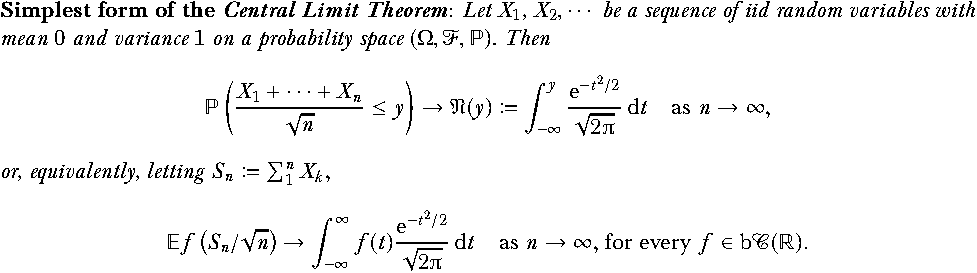
\includegraphics{baskervaldxmatheg-crop}

 
\end{document}  